% Figure floats. Every panel is generated by paper/scripts/make_figures.py from the
% evidence ledger; none is hand-drawn or hand-edited.

\begin{figure}[t]
  \centering
  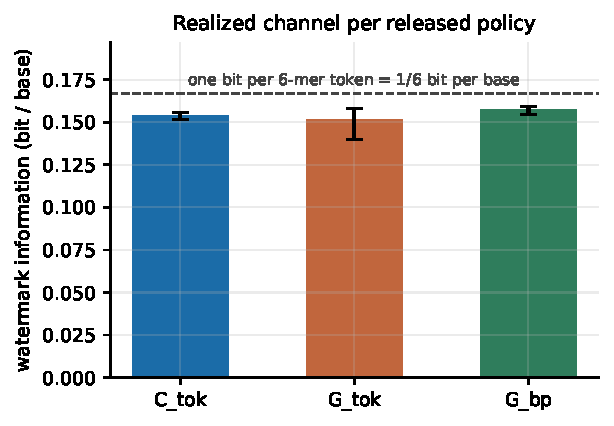
\includegraphics[width=0.62\linewidth]{../../figures/fig01_capacity.pdf}
  \caption{Realized maximal-coupling watermark information per DNA base for the three released
  generation policies, with equal-weight prompt-cluster percentile intervals over the frozen public
  cohort. The dashed line is the construction's structural ceiling of one coupled bit per 6-mer token.}
  \label{fig:capacity}
\end{figure}

\begin{figure}[t]
  \centering
  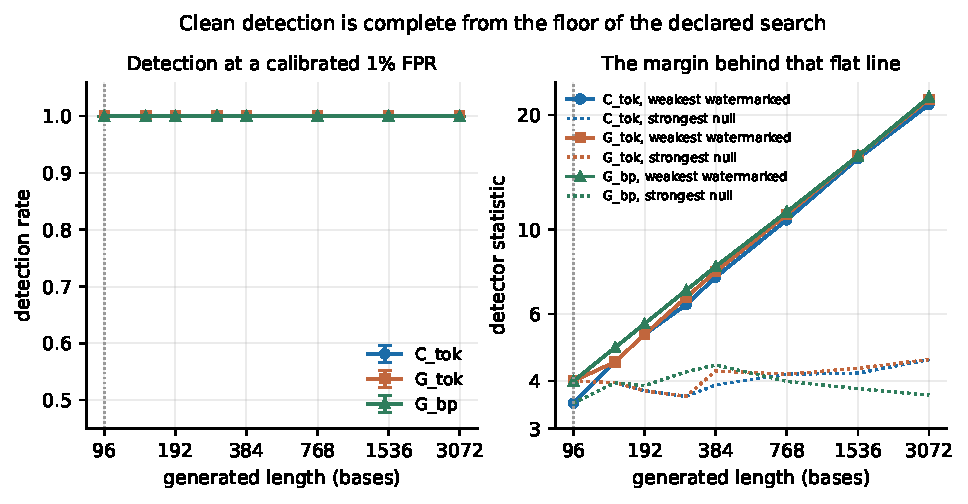
\includegraphics[width=\linewidth]{../../figures/fig02_clean_detection.pdf}
  \caption{Left: correct-key detection rate on clean watermarked DNA against generated length, at a
  false-positive rate calibrated by repeating the identical declared search on null trials. Right: the
  margin behind that flat line. The weakest watermarked statistic and the strongest pooled null
  statistic touch at $\shortestDetectedBases{}$ bases and separate from $\strictSeparationBases{}$
  bases onward, which is why the strict-separation length is admitted separately from the detection
  rate.}
  \label{fig:clean-detection}
\end{figure}

\begin{figure}[t]
  \centering
  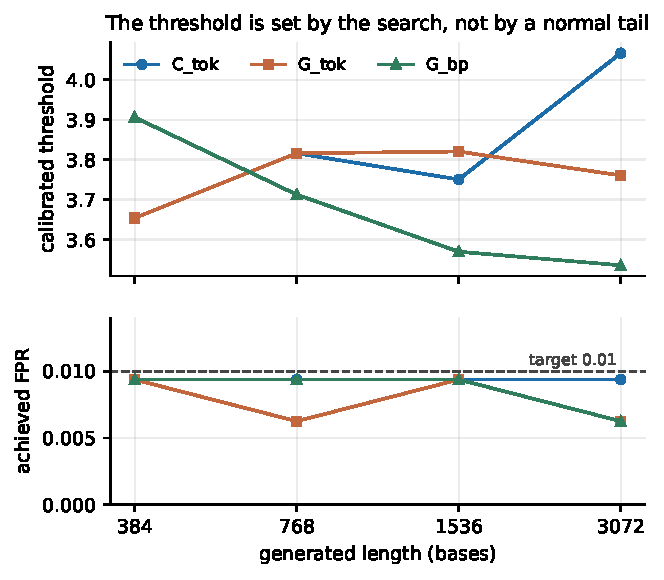
\includegraphics[width=0.62\linewidth]{../../figures/fig03_calibration.pdf}
  \caption{Top: the decision threshold chosen empirically from null trials that repeat the complete
  declared search. Bottom: the false-positive rate that threshold achieves. The reported statistic is a
  maximum over the search, so its nominal normal tail is not a $p$-value and no threshold here comes
  from one.}
  \label{fig:calibration}
\end{figure}

\begin{figure}[t]
  \centering
  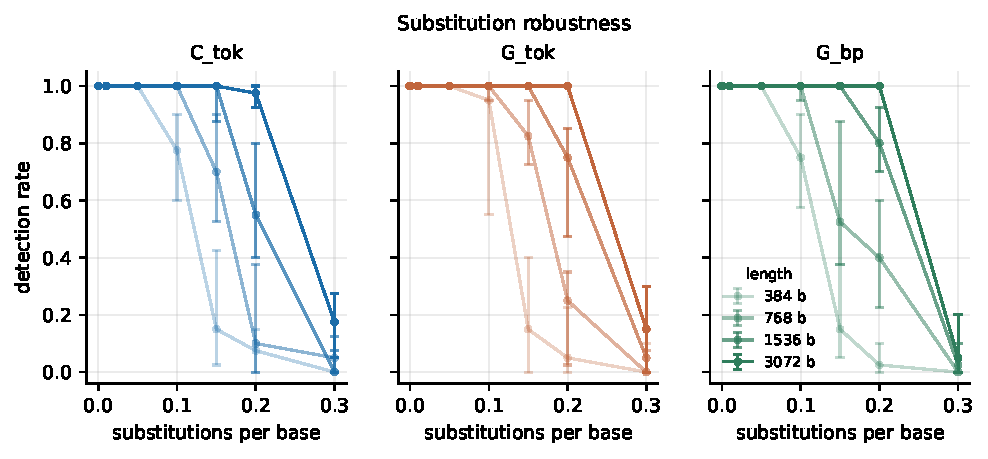
\includegraphics[width=\linewidth]{../../figures/fig04_substitution.pdf}
  \caption{Detection rate against per-base substitution rate, by policy and generated length, at the
  calibrated false-positive rate. Intervals are joint resamples: each replicate resamples the null
  trials, recalibrates the threshold, and independently resamples the prompt clusters.}
  \label{fig:substitution}
\end{figure}

\begin{figure}[t]
  \centering
  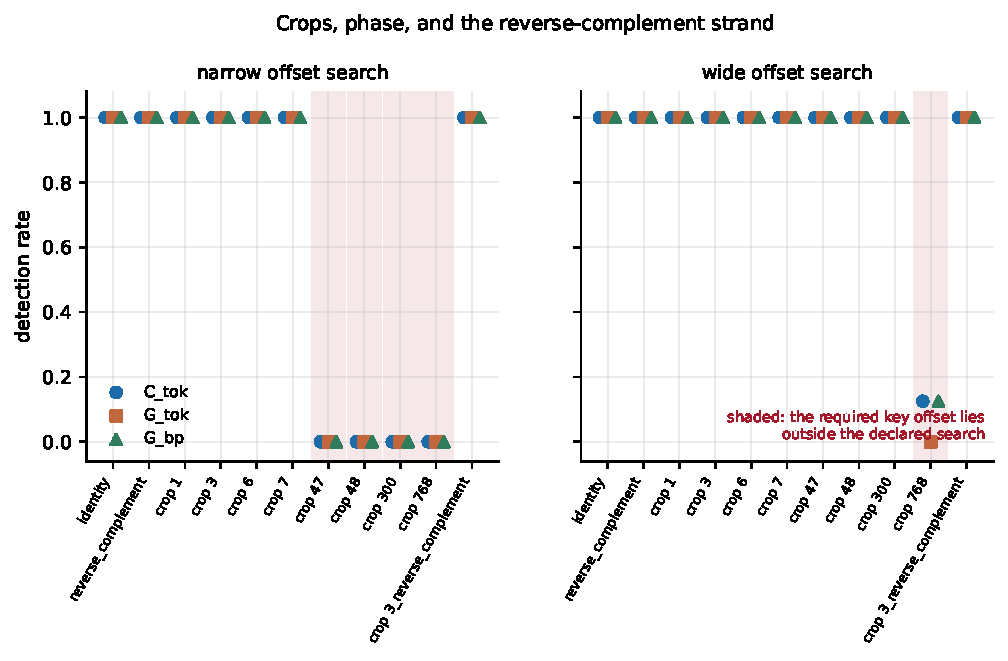
\includegraphics[width=\linewidth]{../../figures/fig05_crop_strand.pdf}
  \caption{Detection per crop, phase, and reverse-complement condition under the narrow and the wide
  declared key-offset search. The three policies agree condition by condition, which is expected rather
  than suspicious: every failing condition, shaded, is one whose required key-stream offset lies
  outside the declared search, a property of the search and not of the model.}
  \label{fig:crop-strand}
\end{figure}

\begin{figure}[t]
  \centering
  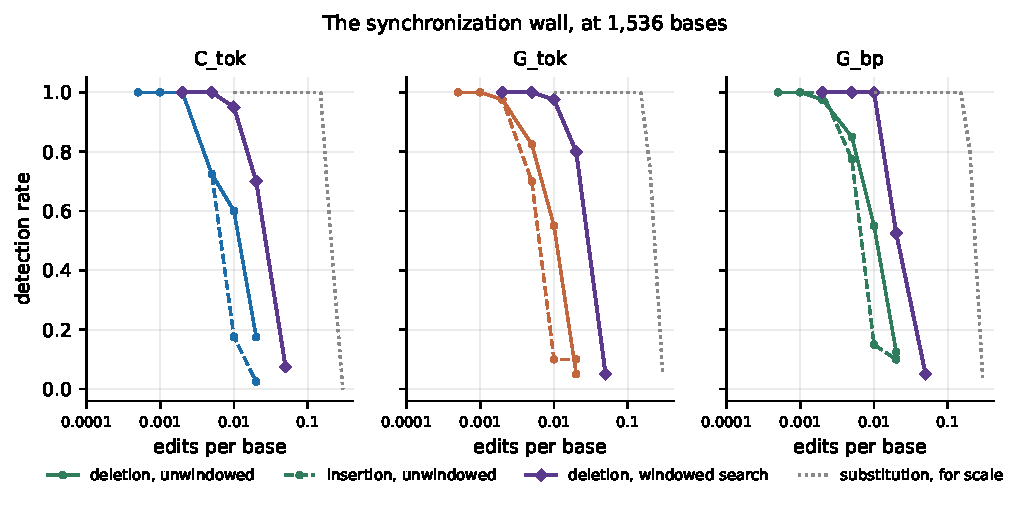
\includegraphics[width=\linewidth]{../../figures/fig06_indel_synchronization.pdf}
  \caption{Detection against per-base edit rate at the longest length the indel experiments evaluated.
  Insertions and deletions defeat the unwindowed detector one to two orders of magnitude below the
  substitution tolerance drawn for scale, because one deleted base moves every later token off the
  reading grid. A declared sliding-window search moves that limit before meeting a second,
  information-theoretic wall.}
  \label{fig:indel}
\end{figure}

\begin{figure}[t]
  \centering
  \includegraphics[width=0.62\linewidth]{../../figures/fig08_baseline_signal_per_token.pdf}
  \caption{Standardized signal per 6-mer token for the three exact-marginal constructions, each in
  units of its own null standard deviation, as a band across the evaluated lengths. Detection rate is
  deliberately not plotted: it is $1.000$ for all three methods at every evaluated length, so plotting
  it would present a null result as agreement. Partition coupling sits at its structural ceiling of one
  coupled bit per token; exponential sampling is not so bounded.}
  \label{fig:baselines}
\end{figure}

\begin{figure}[t]
  \centering
  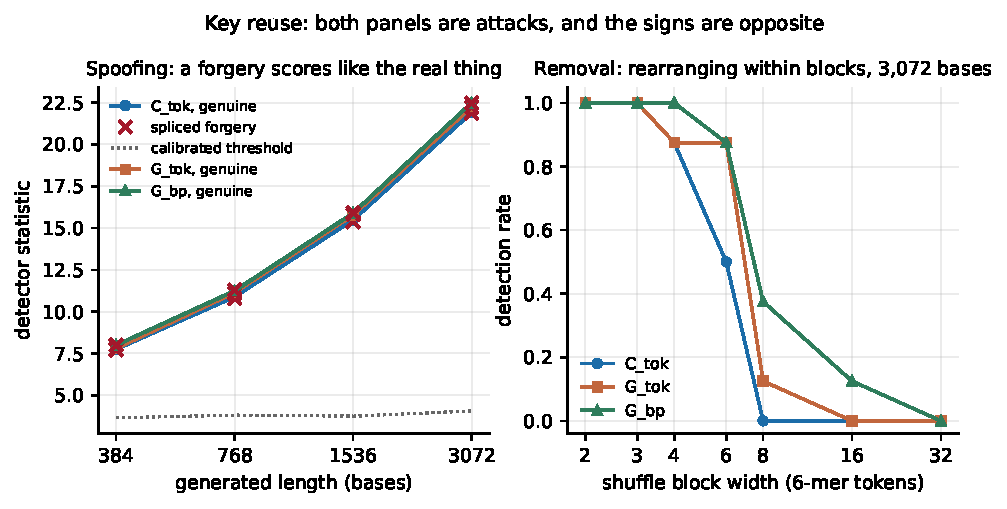
\includegraphics[width=\linewidth]{../../figures/fig09_key_reuse_attacks.pdf}
  \caption{Key reuse. Both panels are attacks and their signs are opposite. Left: a sequence spliced
  position-wise from two watermarked outputs under one key scores indistinguishably from genuine output
  at every length, so the verifier accepts it every time; a high value here is a \emph{vulnerability},
  because the statistic is a sum of content-blind per-position checks and nothing binds a sequence to
  itself. Right: detection after permuting 6-mer positions within blocks of the given width; a low
  value here is a \emph{successful removal}, and it must be read with the proxy cost, because the
  attack preserves the 6-mer multiset exactly and the admitted composition proxies are nearly blind to
  it.}
  \label{fig:attacks}
\end{figure}

\begin{figure}[t]
  \centering
  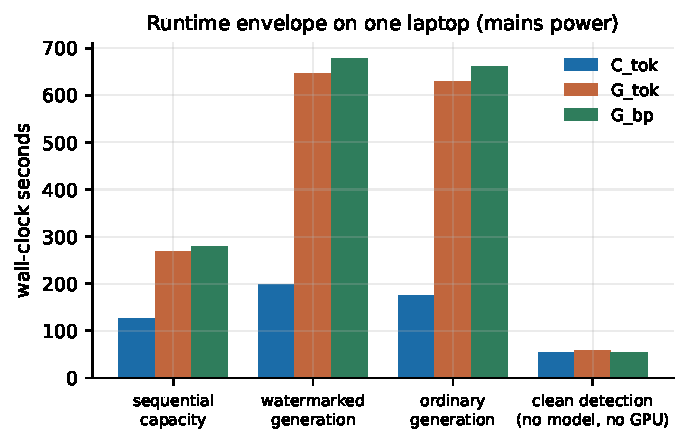
\includegraphics[width=0.62\linewidth]{../../figures/fig07_runtime.pdf}
  \caption{Wall-clock time per stage for one policy on one laptop, from single observations under
  uncontrolled desktop load and on mains power: a feasibility envelope, not a benchmark. No memory
  panel is shown because no peak-memory figure is admitted. Detection uses neither the model nor the
  GPU.}
  \label{fig:runtime}
\end{figure}

\begin{figure}[t]
  \centering
  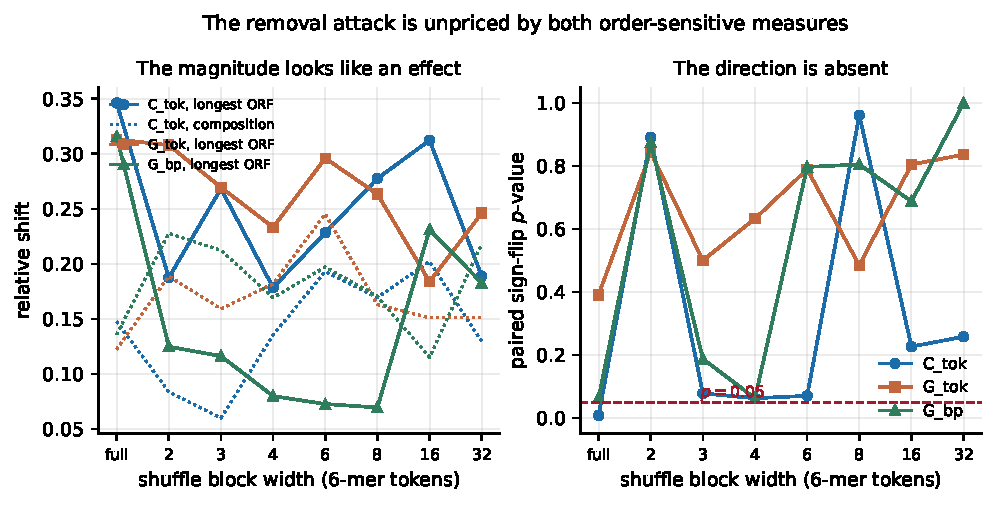
\includegraphics[width=\linewidth]{../../figures/fig10_unpriced_removal.pdf}
  \caption{Why the removal attack remains unpriced. Left: the relative shift of the longest open
  reading frame under each bounded rearrangement, with the largest composition-proxy shift beside it;
  the reading-frame shift is the larger of the two on most cells, which looks like an instrument that
  prices the attack. Right: the exact paired sign-flip $p$-value over the eight prompts for the same
  cells. Only the complete shuffle on one policy shows a directionally consistent change, and under
  every bounded shuffle the longest reading frame rises about as often as it falls --- on high-entropy
  DNA it is a chance extreme-value statistic that a permutation re-rolls rather than destroys. A large
  left-panel value is not evidence of an effect unless the right panel falls below the line.}
  \label{fig:unpriced}
\end{figure}
